%\RequirePackage{lineno}\linenumbers\newdimen\linenumbersep\linenumbersep=2pt
\documentclass[prd,aps,twocolumn,superscriptaddress,showpacs,showkeys,amsmath,amssymb,floatfix]{revtex4}
\usepackage[colorlinks=true,citecolor=blue,filecolor=blue,linkcolor=blue,urlcolor=blue,pdftex]{hyperref}

\usepackage{xspace} 
\usepackage[usenames,dvipsnames]{color}
\usepackage{booktabs,graphicx,mathrsfs,verbatim,amsmath,units,soul}
\usepackage{xspace} 
\usepackage{upgreek}
\usepackage{gensymb}
\usepackage{amsmath}
\usepackage{tabularx}

\sloppy

% NUMBERS

%% **********************
%Intro
%% **********************
\newcommand{\ton}{t}
% total mass LXe
\newcommand{\nxenontotalmass}{$3.2$\;\ton\xspace}
% target mass LXe
\newcommand{\nxenontargetmass}{$2.00$\;\ton\xspace}
% distance cathode to gate
\newcommand{\ntpcdriftlength}{$97~\mathrm{cm}$\xspace}
% diameter of TPC
\newcommand{\ntpcdiameter}{$96~\mathrm{cm}$\xspace}
% extraction field in V/cm
% https://xe1t-wiki.lngs.infn.it/doku.php?id=xenon:xenon1t:julien:xenon1t_3d_field_simulation#s1-region_-_sr1
%  ^ Warning: seems incorrect...
\newcommand{\nextractionfield}{$\sim$4~kV/cm\xspace}
\newcommand{\nmultiplicationfield}{$\sim$8~kV/cm\xspace}
% X ER rejection at Y NR acceptance
\newcommand{\nerrejectionpct}{99.7\%\xspace}
\newcommand{\nnracceptance}{50\%\xspace}
\newcommand{\nxenonnttargetmass}{5.9\;\ton\xspace}

%% **********************
% Detector Parameters 
%% **********************
% Liquid level tolerance
\newcommand{\nliquidleveltolerance}{2\%~RMS\xspace}
% Liquid level above gate
\newcommand{\nliquidlevelabovegate}{$2.5~\mathrm{mm}$\xspace}
% LXe temperature
\newcommand{\nxenoninternaltemp}{$-96.0$\,$^\circ$C\xspace}
% LXe temperature tolerance
\newcommand{\nxenoninternaltemptolerance}{0.02\%~RMS\xspace}
% GXe pressure
\newcommand{\nxenonpressure}{1.94~bar\xspace}
% GXe pressure tolerance
\newcommand{\nxenonpressuretolerance}{0.01\%~RMS\xspace}
% Largest S2 x-y map correction (in middle)
\newcommand{\nlargeststwoxycorrection}{32\%\xspace}
% Drift Fields 
% https://xe1t-wiki.lngs.infn.it/doku.php?id=xenon:xenon1t:jingqiang:field:data_driven_3d_electric_field_map
\newcommand{\driftfieldsrzero}{$120$~V/cm\xspace} %\;\pm\;8
\newcommand{\driftfieldsrone}{$81$~V/cm\xspace} %\;\pm\;7
\newcommand{\driftfielderror}{2.2~V/cm RMS\xspace} %\;\pm\;7

%% **********************
% Livetimes
%% **********************
\newcommand{\SRzero}{SR0\xspace}
\newcommand{\SRone}{SR1\xspace}
% Livetime-corrected SR0
\newcommand{\nlivetimesrzero}{32.1~days\xspace}
% Livetime-corrected SR1
\newcommand{\nlivetimesrone}{246.7~days\xspace}
% Livetime-corrected combined
\newcommand{\nlivetimetotal}{278.8~days\xspace}
% Start date of sciencerun0
\newcommand{\nstartofsciencerunzero}{November~22,~2016\xspace}
% End date of sciencerun1
\newcommand{\nendofsciencerunone}{February~8,~2018\xspace}
% Power outage of sciencerun1
\newcommand{\npoweroutsciencerunone}{February~24,~2018\xspace}
% SR0 DAQ livetime
\newcommand{\ndaqlivetimesrzero}{†92.2\%\xspace}
\newcommand{\ndaqdeadtimesrzero}{7.8\%\xspace}
% SR1 DAQ livetime
\newcommand{\ndaqlivetimesrone}{98.8\%\xspace}
\newcommand{\ndaqdeadtimesrone}{1.2\%\xspace}
% Date of run-ending earthquake
\newcommand{\nearthquakedate}{January~18,~2017\xspace}
% Date SR1 start
\newcommand{\nsronestart}{February~2,~2017\xspace}
% Magnitude of run-ending earthquake
\newcommand{\nearthquakemagnitude}{5.7\xspace}
% Total gain zero PMTs
\newcommand{\nblindedpmts}{36\xspace}
% Gain zero PMTs due to leaks
\newcommand{\nleakypmts}{26\xspace}
% Gain zero PMTs not due to leaks (should add up to total)
\newcommand{\notherpmts}{6\xspace}
% Days lost from muon veto cut
\newcommand{\nlossmuon}{1.2\%\xspace}%{3.4~days\xspace}
% Days lost from PMT flash cut
\newcommand{\nlossflash}{0.2\%\xspace}%{0.6~days\xspace}
% Days lost from S2 tail cut
\newcommand{\nlosstails}{4.4\%\xspace}%{12.3~days\xspace}
% Days of good Rn220 data
\newcommand{\ndaysrn}{17.1 days\xspace}
% Days of good AmBe data
\newcommand{\ndaysambe}{30.0 days\xspace}
% Days of good NG data
\newcommand{\ndaysng}{1.9 days\xspace}

%% **********************
% Thresholds and acceptance
%% **********************
% S2 threshold above 200pe
\newcommand{\nstwoaccoverthresh}{unity\xspace}
% Mean SPE acceptance, 3% is the 1-sigma. RMS would be 9.2%
\newcommand{\nmeanspeacceptance}{$(93\pm3)$\%\xspace}

%% **********************
% Fiducial and backgrounds
%% **********************
% Fiducial mass
\newcommand{\ncoremassname}{0.65~\ton\xspace}
\newcommand{\nonetonnemassname}{0.9~\ton\xspace}
\newcommand{\nnominalfiducialmassname}{1.3~\ton\xspace}
\newcommand{\nnominalfiducialmass}{$(1.30~\pm~0.01)$\;\ton\xspace}
%\newcommand{\nfiducialmass}{$1.6$}
% Combined exposure
\newcommand{\nexposure}{1.0\;\ton$\times$yr\xspace}
% Total NR background in fiducial mass
\newcommand{\ntotalnrbackground}{$XX$}
% Total ER background in fiducial mass
\newcommand{\nwallbackground}{$XX$}
% Kr85 level
\newcommand{\nkrlevel}{$^\mathrm{nat}\mathrm{Kr}/\mathrm{Xe} = (0.66\pm0.11)~\mathrm{ppt}$}
\newcommand{\krrate}{$(7.7\pm 1.3)$~events/$(\mathrm{\ton}\times\mathrm{yr}\times\kevee)$}

\newcommand{\rnlevel}{$(12.6 \pm 0.8)~\mu\mathrm{Bq}/\mathrm{kg}$\xspace}

\newcommand{\rnrate}{$(7.7\pm 1.8)$~events/$(\mathrm{\ton}\times\mathrm{yr}\times\kevee)$}

%\newcommand{\nkrlevel}{$^{85}\mathrm{Kr}/^{nat}\mathrm{Kr} = (1.645 \substack{+0.413 \\ -0.276})\times 10^{-11}$}
% Rn222 level
\newcommand{\nrnlevel}{YY}
%\newcommand{\nlowestbg}{${(63~\pm~2)}$~\dru\xspace}
\newcommand{\nlowestbg}{$(82\substack{+5 \\ -3}\textrm{~(sys)}\pm3\textrm{~(stat)})$~\dru\xspace}

\newcommand{\rntwo}{${}^{222}$Rn\xspace}
\newcommand{\rnzero}{${}^{220}$Rn\xspace}
\newcommand{\krbkg}{${}^{85}$Kr\xspace}
\newcommand{\krm}{${}^{83\mathrm{m}}$Kr\xspace}
\newcommand{\ambe}{${}^{241}$AmBe\xspace} 

\newcommand{\cSone}{$\mathrm{cS1}$\xspace}
\newcommand{\cStwo}{$\mathrm{cS2}$\xspace}
\newcommand{\cStwob}{$\mathrm{cS2_b}$\xspace}
\newcommand{\ucSone}{$\mathrm{S1}$\xspace}
\newcommand{\ucStwo}{$\mathrm{S2}$\xspace}
\newcommand{\Sone}{$\mathrm{S1}$\xspace}
\newcommand{\Stwo}{$\mathrm{S2}$\xspace}
\newcommand{\z}{Z\xspace}
\newcommand{\radius}{R\xspace}
\newcommand{\radiussquared}{R$^{2}$\xspace}

\newcommand{\nmoststringentlimit}{$4.1\times10^{-47}$~cm$^2$\xspace}
\newcommand{\nmoststingentmass}{30~\gevcsq}
\newcommand{\nbestfitsigmasi}{$2.9\times10^{-48}$~cm$^2$\xspace}
\newcommand{\nbestfitsigmasitwoh}{$4.7\times10^{-47}$~cm$^2$\xspace}

\newcommand\figref[1]{Fig.~\ref{#1}}
\newcommand\Figref[1]{Figure~\ref{#1}}
\newcommand\tabref[1]{Table~\ref{#1}}
\newcommand\figsref[2]{Figs.~\ref{#1}~and~\ref{#2}}
\newcommand\Figsref[2]{Figures~\ref{#1}~and~\ref{#2}}

\newcommand{\kevee}{\mathrm{keV_{ee}}}
\newcommand{\kevnr}{\mathrm{keV_{nr}}}

% Old abbreviations
\newcommand{\AC}{AC\xspace}
\newcommand{\FM}{fiducial mass\xspace}

% old microscopic units
%\newcommand{\dru}{($\mathrm{kg}\times\mathrm{day}\times\mathrm{keV})^{-1}$\xspace}
% new macroscopic units
\newcommand{\dru}{events/$(\mathrm{\ton}\times\mathrm{yr}\times\kevee)$}
\newcommand{\gevcsq}{GeV/c${}^2$\xspace}
\newcommand{\tevcsq}{TeV/c${}^2$\xspace}
\newcommand{\searchregion}{cS$1\!\in\![3, 70]\;\mathrm{PE}$, cS$2_b\!\in\![50, 8000]\;\mathrm{PE}$~search region}
% https://xe1t-wiki.lngs.infn.it/doku.php?id=greene:bbf_acceptances
\newcommand{\searchregionkev}{[1.4,~10.6]~$\kevee$\xspace}
\newcommand{\searchregionkevnr}{[4.9,~40.9]~$\kevnr$\xspace}

\newcommand{\todo}[1]{\textcolor{red}{\textbf{$\lceil$#1$\rfloor$}}}
\newcommand{\num}[1]{#1}

\newcommand{\red}[1]{\textcolor{red}{#1}}
\newcommand{\arxiv}[1]{\href{http://arxiv.org/abs/#1}{\texttt{arXiv:#1}}}

\makeatletter
\newcommand{\romenum}[1]{(\romannumeral #1)}
\makeatother

\newcommand{\Delete}[2][magenta]{\textcolor{#1}{\sout{#2}}}
\newcommand{\Modify}[2][magenta]{\textcolor{#1}{\textrm{#2}}}

\newcommand{\bern}{\affiliation{Albert Einstein Center for Fundamental Physics, University of Bern, 3012 Bern, Switzerland}}

\newcommand{\bologna}{\affiliation{Department of Physics and Astronomy, University of Bologna and INFN-Bologna, 40126 Bologna, Italy}}

\newcommand{\chicago}{\affiliation{Department of Physics \& Kavli Institute for Cosmological Physics, University of Chicago, Chicago, IL 60637, USA}}

\newcommand{\coimbra}{\affiliation{LIBPhys, Department of Physics, University of Coimbra, 3004-516 Coimbra, Portugal}}

\newcommand{\columbia}{\affiliation{Physics Department, Columbia University, New York, NY 10027, USA}}

\newcommand{\lngs}{\affiliation{INFN-Laboratori Nazionali del Gran Sasso and Gran Sasso Science Institute, 67100 L'Aquila, Italy}}

\newcommand{\mainz}{\affiliation{Institut f\"ur Physik \& Exzellenzcluster PRISMA, Johannes Gutenberg-Universit\"at Mainz, 55099 Mainz, Germany}}

\newcommand{\heidelberg}{\affiliation{Max-Planck-Institut f\"ur Kernphysik, 69117 Heidelberg, Germany}}

\newcommand{\munster}{\affiliation{Institut f\"ur Kernphysik, Westf\"alische Wilhelms-Universit\"at M\"unster, 48149 M\"unster, Germany}}

\newcommand{\nikhef}{\affiliation{Nikhef and the University of Amsterdam, Science Park, 1098XG Amsterdam, Netherlands}}

\newcommand{\nyuad}{\affiliation{New York University Abu Dhabi, Abu Dhabi, United Arab Emirates}}

\newcommand{\purdue}{\affiliation{Department of Physics and Astronomy, Purdue University, West Lafayette, IN 47907, USA}}

\newcommand{\rpi}{\affiliation{Department of Physics, Applied Physics and Astronomy, Rensselaer Polytechnic Institute, Troy, NY 12180, USA}}

\newcommand{\rice}{\affiliation{Department of Physics and Astronomy, Rice University, Houston, TX 77005, USA}}

\newcommand{\stockholm}{\affiliation{Oskar Klein Centre, Department of Physics, Stockholm University, AlbaNova, Stockholm SE-10691, Sweden}}

\newcommand{\subatech}{\affiliation{SUBATECH, IMT Atlantique, CNRS/IN2P3, Universit\'e de Nantes, Nantes 44307, France}}

\newcommand{\torino}{\affiliation{INFN-Torino and Osservatorio Astrofisico di Torino, 10125 Torino, Italy}}

\newcommand{\ucla}{\affiliation{Physics \& Astronomy Department, University of California, Los Angeles, CA 90095, USA}}

\newcommand{\ucsd}{\affiliation{Department of Physics, University of California, San Diego, CA 92093, USA}}

\newcommand{\wis}{\affiliation{Department of Particle Physics and Astrophysics, Weizmann Institute of Science, Rehovot 7610001, Israel}}

\newcommand{\zurich}{\affiliation{Physik-Institut, University of Zurich, 8057  Zurich, Switzerland}}

\newcommand{\paris}{\affiliation{LPNHE, Universit\'{e} Pierre et Marie Curie, Universit\'{e} Paris Diderot, CNRS/IN2P3, Paris 75252, France}}

\newcommand{\freiburg}{\affiliation{Physikalisches Institut, Universit\"at Freiburg, 79104 Freiburg, Germany}}



\begin{document}

% CHANGE TO TITLE

\title{Background Modeling and Statistical Inference for WIMP Searches in XENON1T }

\author{E.~Aprile}\columbia
\author{J.~Aalbers}\nikhef
\author{F.~Agostini}\bologna
\author{M.~Alfonsi}\mainz
\author{L.~Althueser}\munster
\author{F.~D.~Amaro}\coimbra
\author{M.~Anthony}\columbia
\author{F.~Arneodo}\nyuad
\author{L.~Baudis}\zurich
\author{B.~Bauermeister}\stockholm
\author{M.~L.~Benabderrahmane}\nyuad
\author{T.~Berger}\rpi
\author{P.~A.~Breur}\nikhef
\author{A.~Brown}\nikhef
\author{A.~Brown}\zurich
\author{E.~Brown}\rpi
\author{S.~Bruenner}\heidelberg
\author{G.~Bruno}\nyuad
\author{R.~Budnik}\wis
\author{C.~Capelli}\zurich
\author{J.~M.~R.~Cardoso}\coimbra
\author{D.~Cichon}\heidelberg
\author{D.~Coderre}\freiburg
\author{A.~P.~Colijn}\nikhef
\author{J.~Conrad}\stockholm
\author{J.~P.~Cussonneau}\subatech
\author{M.~P.~Decowski}\nikhef
\author{P.~de~Perio}\columbia
\author{P.~Di~Gangi}\bologna
\author{A.~Di~Giovanni}\nyuad
\author{S.~Diglio}\subatech
\author{A.~Elykov}\freiburg
\author{G.~Eurin}\heidelberg
\author{J.~Fei}\ucsd
\author{A.~D.~Ferella}\stockholm
\author{A.~Fieguth}\munster
\author{W.~Fulgione}\lngs\torino
\author{A.~Gallo Rosso}\lngs
\author{M.~Galloway}\zurich
\author{F.~Gao}\columbia
\author{M.~Garbini}\bologna
\author{C.~Geis}\mainz
\author{L.~Grandi}\chicago
\author{Z.~Greene}\columbia
\author{H.~Qiu}\wis
\author{C.~Hasterok}\heidelberg
\author{E.~Hogenbirk}\nikhef
\author{J.~Howlett}\columbia
\author{R.~Itay}\wis
\author{F.~Joerg}\heidelberg
\author{B.~Kaminsky}\altaffiliation[Also at ]{Albert Einstein Center for Fundamental Physics, University of Bern, Bern, Switzerland}\freiburg
\author{S.~Kazama}\altaffiliation[Also at ]{Kobayashi-Maskawa Institute, Nagoya University, Nagoya, Japan}\zurich
\author{A.~Kish}\zurich
\author{G.~Koltman}\wis
\author{H.~Landsman}\wis
\author{R.~F.~Lang}\purdue
\author{L.~Levinson}\wis
\author{Q.~Lin}\columbia
\author{S.~Lindemann}\freiburg
\author{M.~Lindner}\heidelberg
\author{F.~Lombardi}\ucsd
\author{J.~A.~M.~Lopes}\altaffiliation[Also at ]{Coimbra Polytechnic - ISEC, Coimbra, Portugal}\coimbra
\author{J.~Mahlstedt}\stockholm
\author{A.~Manfredini}\wis 
\author{T.~Marrod\'an~Undagoitia}\heidelberg
\author{J.~Masbou}\subatech
\author{D.~Masson}\purdue
\author{M.~Messina}\nyuad
\author{K.~Micheneau}\subatech
\author{K.~Miller}\chicago
\author{A.~Molinario}\lngs
\author{K.~Mor\aa}\stockholm
\author{M.~Murra}\munster
\author{J.~Naganoma}\rice
\author{K.~Ni}\ucsd
\author{U.~Oberlack}\mainz
\author{B.~Pelssers}\stockholm
\author{F.~Piastra}\zurich
\author{J.~Pienaar}\chicago
\author{V.~Pizzella}\heidelberg
\author{G.~Plante}\columbia
\author{R.~Podviianiuk}\lngs
\author{N.~Priel}\wis
\author{D.~Ram\'irez~Garc\'ia}\freiburg
\author{L.~Rauch}\heidelberg
\author{S.~Reichard}\zurich
\author{C.~Reuter}\purdue
\author{B.~Riedel}\chicago
\author{A.~Rizzo}\columbia
\author{A.~Rocchetti}\freiburg
\author{N.~Rupp}\heidelberg
\author{J.~M.~F.~dos~Santos}\coimbra
\author{G.~Sartorelli}\bologna
\author{M.~Scheibelhut}\mainz
\author{S.~Schindler}\mainz
\author{J.~Schreiner}\heidelberg
\author{D.~Schulte}\munster
\author{M.~Schumann}\freiburg
\author{L.~Scotto~Lavina}\paris
\author{M.~Selvi}\bologna
\author{P.~Shagin}\rice
\author{E.~Shockley}\chicago
\author{M.~Silva}\coimbra
\author{H.~Simgen}\heidelberg
\author{D.~Thers}\subatech
\author{F.~Toschi}\bologna\freiburg
\author{G.~Trinchero}\torino
\author{C.~Tunnell}\chicago
\author{N.~Upole}\chicago
\author{M.~Vargas}\munster
\author{O.~Wack}\heidelberg
\author{H.~Wang}\ucla
\author{Z.~Wang}\lngs
\author{Y.~Wei}\ucsd
\author{C.~Weinheimer}\munster
\author{C.~Wittweg}\munster
\author{J.~Wulf}\zurich
\author{J.~Ye}\ucsd
\author{Y.~Zhang}\columbia
\author{T.~Zhu}\columbia
\collaboration{XENON Collaboration}
\email[]{xenon@lngs.infn.it}
\noaffiliation

\date{\today} 

\begin{abstract}

\end{abstract}


\pacs{
    95.35.+d, %Dark matter
    14.80.Ly, %Supersymmetric partners of known particles
    29.40.-n,  %Radiation detectors
    95.55.Vj
}

\keywords{Dark Matter, Direct Detection, Xenon, Data Analysis}

\maketitle

\section{Introduction}
% @all

\section{Detector Signal Response Model}
% @Qing





XENON1T WIMP signal and background model used in the statistical inference are built based on the simulation which takes into consideration the detailed characterizations of the detector systematics, as well as the most comprehensible modeling of the recombination process of the liquid xenon.
The coherent modeling of the electronic recoils (ERs) and nuclear recoils (NR) is of high accuracy in terms of the uncertainty of the nuisance parameters and their correlations.
In this chapter, the details of the detector signal response model will be given.

\subsection{Basic Signal Response in Liquid Xenon}
% @Qing


\subsection{Recombination in Low Energy}
% @Qing


\subsection{Influence by Detector Reconstruction}
% @Qing

\section{Background and Dark Matter Signal Model}

\subsection{Electronic Recoil Backgrounds}
% @Qing
% Here I think we need to mention a few things: 1: What are the individual components and how are they determined, which I (Fei) can help together with Patrick. 2: How will they distribute in POI, which is Qing's job.
% Yes as we put on the outline docs



\subsection{Nuclear Recoil Backgrounds}
% @?

\subsubsection{Radiogenic Neutrons}
% @?
% Fei: I can write the first version for neutron BG stuff. Probably will have more time during IDM boring talks :) 
% The NR modelling part can be in previous section, similar to the ER part.

\subsubsection{Solar Neutrino}
$\ $
% @Patrick? Someone from neutrino field 



\subsection{Surface Backgrounds}
% @Fei
Just add the content to start, will modify the description further.....

Interactions in the inner part of the detector can be nicely modelled by combining our knowledge on LXe's properties to ionizing particles and the detector related properties like charge/light collections. In cases where the latter information is missing/incomplete, we need to develop new algorithms to model the events. In this and following sections, two classes of background components are analyzed for the XENON1T dark matter searches.

As has been proved by several experiments~\cite{cdms, deap}, detector surfaces exposed long to ambient air during construction phase are contaminated by large amount of radon progeny, in particular the $^{210}$Pb. With a 22\,y half-life, $^{210}$Pb basically decays constantly within the XENON1T's operation of a few years. For dark matter searches, ion recoil of $^{206}$Pb from $^{210}$Po $\alpha$-decays, $\beta$-decays and the resulting X-rays, Auger electrons of $^{210}$Pb are particularly important. Due to unknown LXe's properties and detector physics in presence of PTFE as well as the complicated decay structures, a precise modeling based on Monte-Carlo simulation approach has not been achieved in XENON1T yet. Instead, a data driven approach is adopted to predict the event distribution of this background. 




\begin{figure}[tbp]
\centering
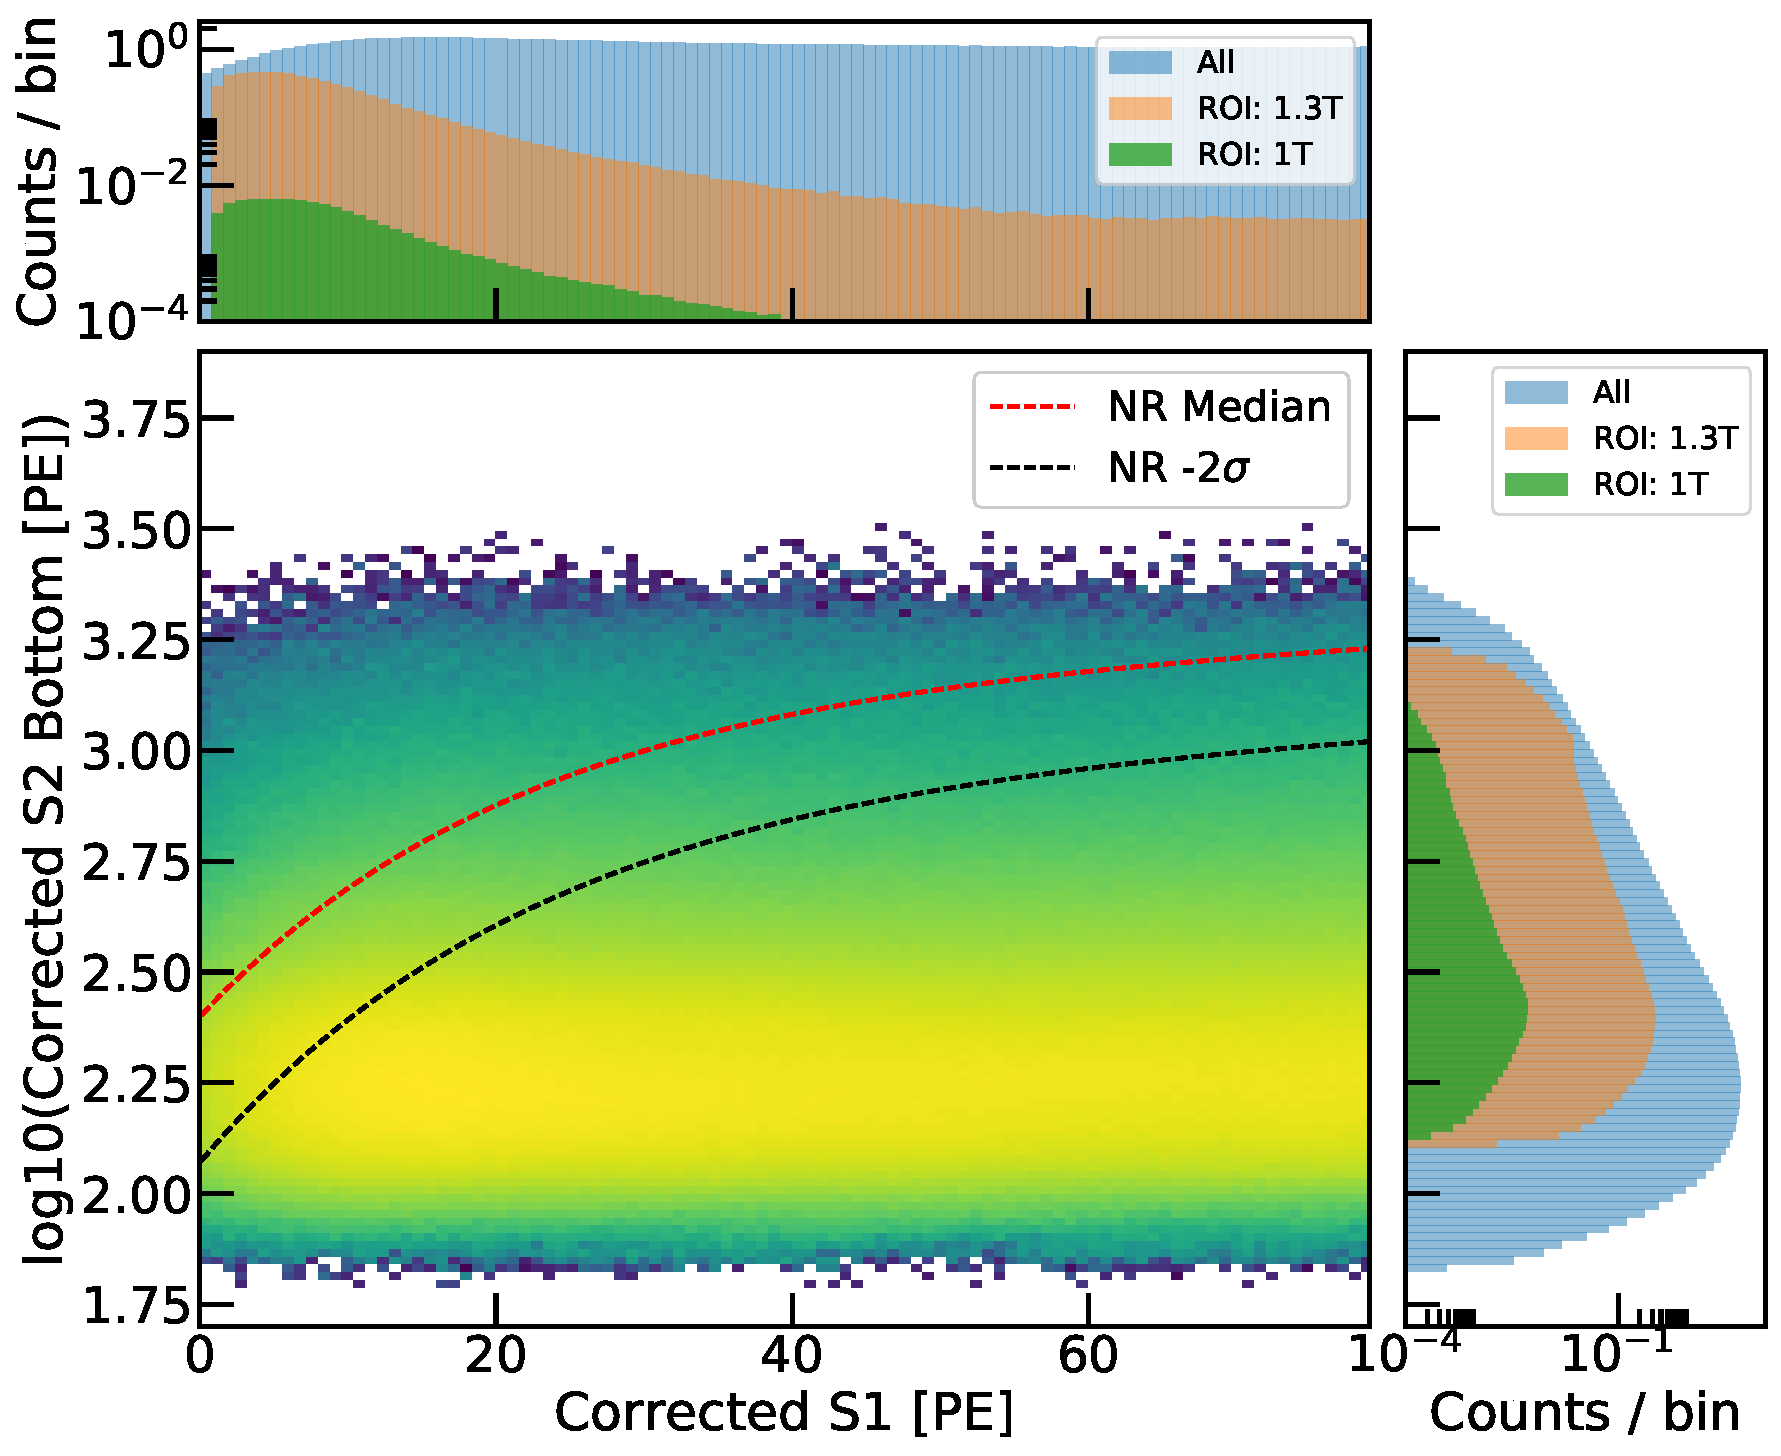
\includegraphics[width=\columnwidth]{Plots/surface_s2s1_distribution_blessed_sr1.pdf}
\caption{\label{fig:surface_bg} 
}
\end{figure}





\subsection{Accidental Pile-up}
% @Fei



\begin{figure}[tbp]
\centering
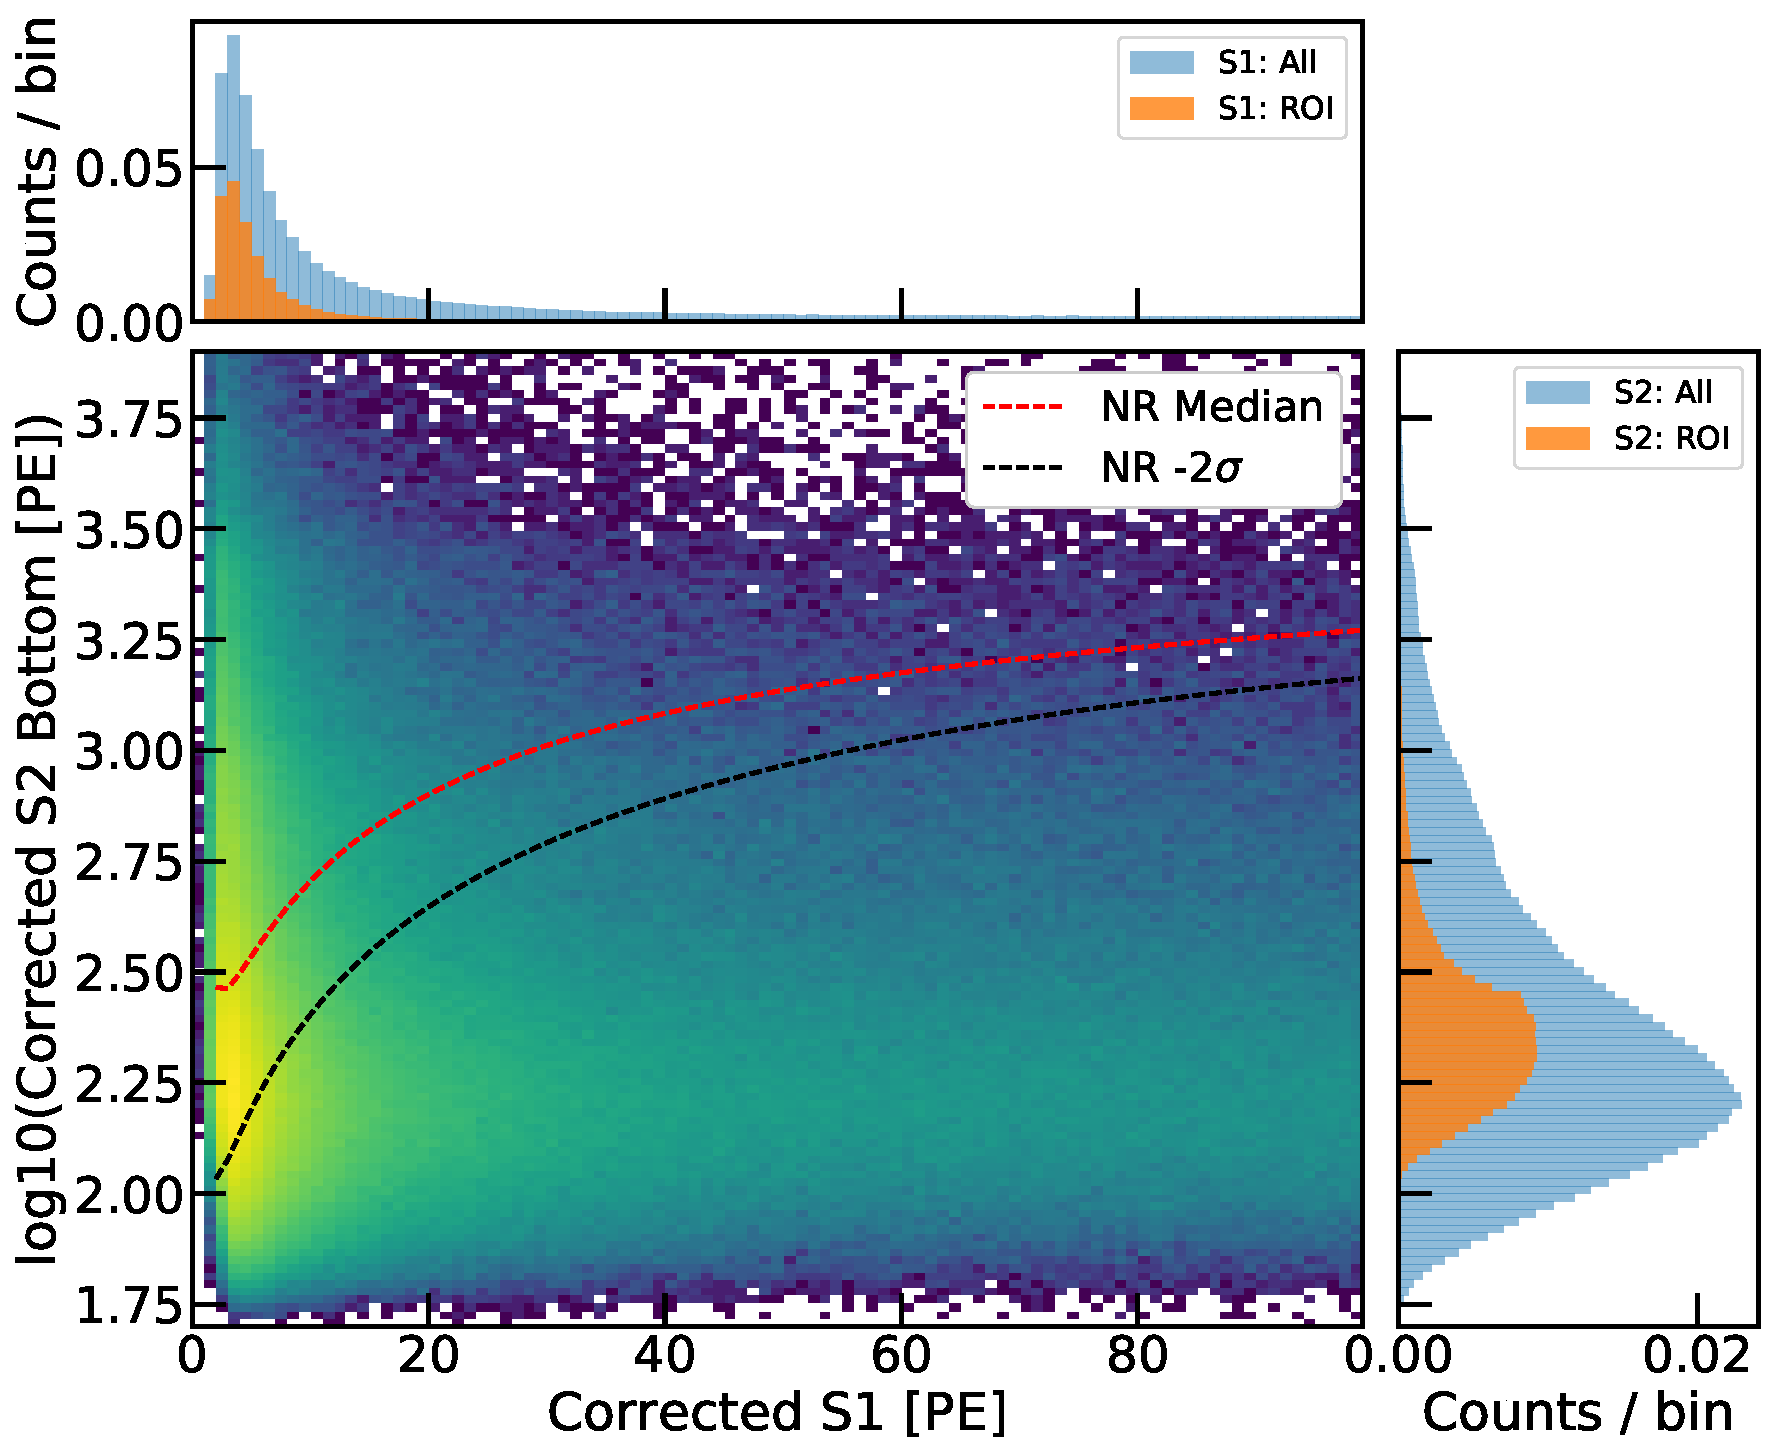
\includegraphics[width=\columnwidth]{Plots/ac_s2s1_distribution_fv1_blessed_sr1.pdf}
\caption{\label{fig:ac_bg} 
}
\end{figure}



\subsection{Dark Matter Signal Model}

\section{Statistical Inference}



\subsection{Inference of XENON1T Data}
\newcommand{\lagr}{\mathcal{L}} %likelihood
\newcommand{\LL}{\log \mathcal{L}} %likelihood
\newcommand{\sr}{\mathrm{SR}}
\newcommand{\nuis}{\theta}
\newcommand{\nuiss}{\vec{\nuis}}
\newcommand{\Pois}[2]{\mathrm{Pois}(#1 | #2)}
\newcommand{\Gaus}[3]{\mathrm{Gaus}(#1 | #2,#3)}
\newcommand{\Uniform}[3]{\mathrm{Uniform}(#1 | #2,#3)}


\subsection{The XENON1T Combined Likelihood}
%Knut
The log-likelihood used in the spin-independent analysis is a sum of extended un-binned likelihoods for the two science runs, extended un-binned likelihoods for ER calibration data, and terms expressing ancillary measurements of nuisance parameters $\nuis_m$: 
\\
Where $\sr$ runs over data-taking periods, \SRzero and \SRone, $\sigma$ is the WIMP-nucleon cross-section, and $\LL_\mathrm{sci}$,$\LL_\mathrm{cal}$ are the likelihood terms for the dark matter search data and \rnzero calibration data, respectively. Ancillary measurements  The un-binned likelihoods take the form: 

\subsection{Analysis Dimensions}
%radial choice
%benefit of less analysis space
%does FV definition go here? 
\subsection{Core Volume Segmentation}

\subsection{Safeguard}
A mismodelling term, proposed in~\cite{safeguard} is added to the ER model, consisting of a signal-like component added or subtracted to the nominal ER model: 


Since the PDF is constrained to be non-negative, the 


\subsection{Nuisance Parameters}
%Mention here: 
%BBF nuisance parameter propagation
%Radiogenics common parameter, others uncorrelated
%wall shape parameter consideration
%why signal shape was dropped
%signal rate uncertainties


\subsection{Trial Correction}
As discovery significances are computed for WIMP-masses between $6$ and $1000$ GeV, the final p-value of the experiment must reflect that multiple hypotheses were tested, and the lowest local p-value is picked as the most significant excess. The result is correlated between multiple masses, with a lower correlation between the peaked low-mass WIMP, and complete correlation between dark matter masses above $~200$ GeV, where the recoil spectrum converges. Toy Monte-Carlo data samples are generated without a dark matter signal, and discovery significances are computed for the entire mass range. The lowest local p-value is stored to compute the distribution of most significant local p-values. The global significance of the actual dataset is the percentile of the lowest p-value from the actual data of this distribution. Using local p-values rather than log-likelihood rations directly corrects for the uneven weighting that would result as different masses do not have the same null-distribution of the discovery log-likelihood ratio.


\subsection{Coverage}
The fraction of repeated experiments where the confidence interval contains the true parameter is called the coverage. Perfect coverage is equal to the confidence interval, $0.9$ in the case of XENON. As the experiment decided to report only the upper edge of the confidence interval for discovery significances $<3\sigma$, there will be over-coverage at very low signal sizes. This has a similar effect to the power constraint. Figure~\ref{fig:coverage}n shows the coverage for a $50$ GeV WIMP, with the red line representing the profile construction coverage, and blue the coverage including the $3\sigma$ threshold. The orange band, shows the $-\sigma$ to $\sigma$ sensitivity band. The result is consistent with perfect coverage (marked by the gray band, including limited statistics), with overcoverage for the $3\sigma$ threshold only under the $-1\sigma$ edge of the sensitivity band. 

\begin{figure}[tbp]
\centering
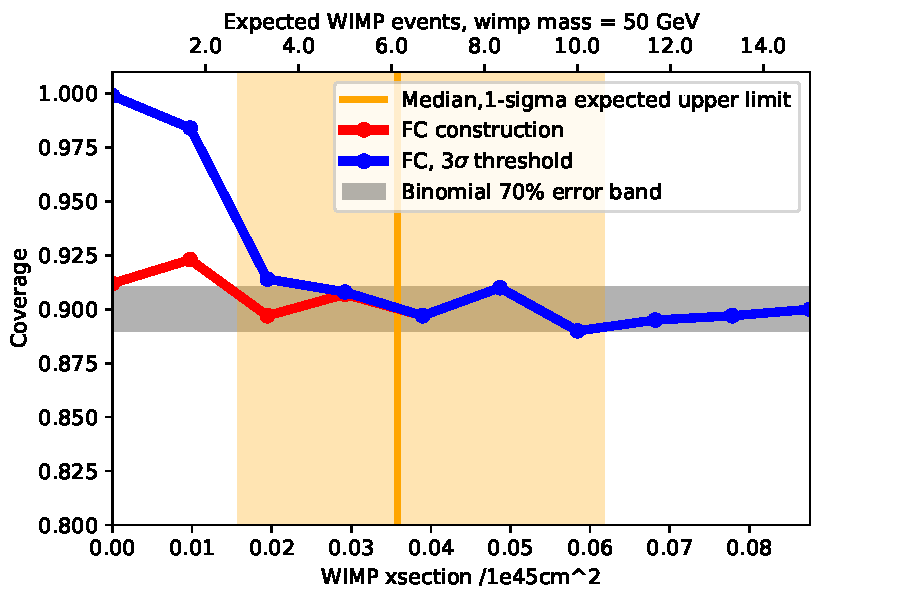
\includegraphics[width=\columnwidth]{{Plots/blueice_coverage_FCplus3sigma_wimp_mass50_livetime278.87151m}.pdf}
\caption{\label{fig:coverage} 
}
\end{figure}

 



\begin{thebibliography}{24}
\addcontentsline{toc}{chapter}{Bibliography} 

\bibitem{wimp_hooper} G.~Bertone, D.~Hooper and J.~Silk, Phys. Rep. \textbf{405}, 279 (2005).

\bibitem{wimp_review} L.~Roszkowski {\it et al.} Rep. Prog. Phys. \textbf{81}, 066201 (2018). %[arXiv:1707.06277]

\bibitem{teresa_review} T.~Marrod\'an Undagoitia and L.~Rauch, J.\ Phys.\ G {\bf 43}, no. 1, 013001 (2016)

\bibitem{indirect} L.~E.~Strigari, Phys. Rep. \textbf{531}, 1 (2012).
%6
\bibitem{xe_sr0} E.~Aprile {\it et al.} (XENON Collaboration), Phys. Rev. Lett. \textbf{119}, 181301 (2017). %[arXiv:1705.06655].
%7
\bibitem{lux_dm} D. S. Akerib {\it et al.} (LUX Collaboration), Phys. Rev. Lett. \textbf{118}, 021303 (2016). %[arXiv:1608.07648].
%8
\bibitem{panda_dm} X. Cui {\it et al.} (PandaX-II Collaboration), Phys. Rev. Lett. \textbf{119}, 181302 (2017). %[arXiv:1708.06917].
%9
\bibitem{xe_instrument} E.~Aprile {\it et al.} (XENON Collaboration), Eur. Phys. J. C \textbf{77}: 881 (2017). %[arXiv:1708.07051].
\bibitem{xe_pmts} E.~Aprile {\it et al.} (XENON Collaboration), Eur. Phys. J. C \textbf{75}: 546 (2015). %[arXiv:1503.07698]. 
\bibitem{pmt2} P. Barrow {\it et al.} JINST \textbf{12}, no. 01, P01024 (2017). % [arXiv:1609.01654].

%10
\bibitem{xe_muonveto} E.~Aprile {\it et al.} (XENON Collaboration), JINST \textbf{9}, P11006 (2014). %[arxiv:1406.2374].

\bibitem{sorensen} P.~Sorensen, K.~Kamdin. JINST \textbf{13}, P02032 (2018). %[arxiv:1711.07025].

\bibitem{kemfield} D.~Furse {\it et al.}. New J. Phys. \textbf{19} 053012 (2017)

\bibitem{luxkr} D. S. Akerib {\it et al.}, Phys. Rev. D \textbf{96}, 112009 (2017). % [arXiv:1708.02566].

% rn220
\bibitem{xe_rn220} E.~Aprile {\it et al.} (XENON Collaboration), Phys. Rev. D \textbf{95}, 072008 (2017).

%11
\bibitem{xe1t_ng} R.~F.~Lang {\it et al.}, Nucl. Inst. and Meth. A \textbf{879}, 31 (2018).

\bibitem{pearc_computing} B. Riedel {\it et al.} PEARC '18, ISBN 978-1-4503-6446-1 (2018). doi:10.1145/3219104.3219155.

\bibitem{pax} XENON Collaboration. (2018). The pax data processor v6.8.0. Zenodo. http://doi.org/10.5281/zenodo.1195785
%14
\bibitem{pmt_calibration} R.~Saldanha {\it et al.}, Nucl. Inst. and Meth. A \textbf{863}, 35 (2017). %[arXiv:1602.03150].
%15
\bibitem{double_pe} C. H. Faham {\it et al.}, JINST \textbf{10}, P09010 (2015).


\bibitem{lux_field} D. S. Akerib {\it et al.} (LUX Collaboration), JINST \textbf{12}, P11022 (2017).

\bibitem{lewin} J. Lewin and P. Smith, Astropart. Phys. \textbf{6} 87 (1996).

\bibitem{xe_kr} E.~Aprile {\it et al.} (XENON Collaboration), Eur. Phys. J. C \textbf{77}: 275 (2017). %[arXiv:1612.04284].
%16
\bibitem{xe_sebastian} S. Lindemann, H. Simgen, Eur. Phys. J. C \textbf{74}, 2746 (2014). %[arXiv:1308.4806].

\bibitem{xe_rn} E.~Aprile {\it et al.} (XENON Collaboration),	Eur. Phys. J. C \textbf{78} :132 (2018). %[arXiv:1708.03617]

%17
\bibitem{solarflux} A.~M.~Serenelli {\it et al.}, Astro. Phys. Journal \textbf{743}, 29 (2011). %[arXiv:1104.1639].
%18
\bibitem{coherent} D.~Akimov {\it et al.} (COHERENT Collaboration), Science \textbf{357}, 1123-1126 (2017). %[arXiv:1708.01294].

\bibitem{geant4} S.~Agostinelli {\it et al.}, Nucl. Inst. and Meth. A \textbf{506}, 250 (2003).

\bibitem{xenon1t_mc_paper} E.~Aprile {\it et al.} (XENON Collaboration), J.\ Cosmol.\ Astropart.\ Phys. \textbf{1604}, no. 04, 027 (2016)

\bibitem{xe_screen} E.~Aprile {\it et al.} (XENON Collaboration), Eur. Phys. J. C \textbf{77}: 890 (2017). 

\bibitem{sources4a} W.B.~Wilson {\it et al.}, LANL technical note LA-13639-MS (1999). 

\bibitem{mcnpx} R.~Lemrani {\it et al.}, Nucl. Inst. and Meth. A \textbf{560}, 454 (2006). %[arXiv:0601030].

\bibitem{xe100_tritium} E.~Aprile {\it et al.} (XENON Collaboration), Phys. Rev. D \textbf{97}, 092007 (2018). 


\bibitem{ti_model} J. Thomas, and D. A. Imel, Phys. Rev. A \textbf{36}, 614 (1987).

\bibitem{NEST_v1} B. Lenardo {\it et al.} IEEE Trans. Nucl. Sci. \textbf{62}, 3387 (2015).

\bibitem{lux_tritium} D. S. Akerib et al. (LUX Collaboration), Phys. Rev. D \textbf{93}, 072009 (2016).

\bibitem{pixey_ar37} E. M. Boulton {\it et al.}, JINST \textbf{12}, P08004 (2017).

\bibitem{lux_xe127} D. S. Akerib {\it et al.} (LUX Collaboration), Phys. Rev. D \textbf{96}, 112011 (2017).

\bibitem{feldmancousins} G.~J.~Feldman and R.~D.~Cousins, Phys. Rev. D {\bf 57}, 3873 (1998).

\bibitem{PDG} C.~Patrignani {\it et al.} (Particle Data Group), Chin. Phys. C \textbf{40}, 100001 (2016).

\bibitem{James:1980ci} F.~James, Comput.\ Phys.\ Commun.\  \textbf{ 20}, 29 (1980).


\bibitem{Bartlett:1953} M. S. Bartlett, Biometrika \textbf{40} 3/4 (1953).

\bibitem{safeguard} N. Priel, L. Rauch, H. Landsman, A. Manfredini, and R. Budnik, J.\ Cosmol.\ Astropart.\ Phys. \textbf{5} 13 (2017). 

\bibitem{exo_nature} J.~B.~Albert {\it et al.} (EXO-200 Collaboration), Nature \textbf{510}, 225 (2014). 

\end{thebibliography}
\end{document}
